\section{2006 - PHYSICS 2A ALTERNATIVE A PRACTICAL}

\begin{enumerate}
\item[1.] In this experiment you are required to determine the mass of unknown object ``X''.

\begin{center}
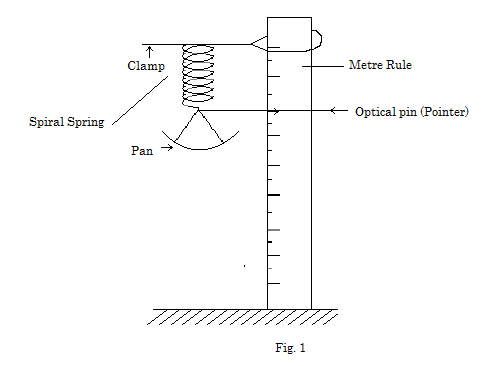
\includegraphics[width=10cm]{./img/2006-1-alt.png}
\end{center}

Assemble the pieces of apparatus as shown in Figure 1, with zero mark scale of the rule at the lower most end.\\

Record the reading of the position of pointer on the scale of metre-rule when the pan is empty as $S_0$.\\

Put 20 g to the pan and record pointer reading $S$.\\

Find extension $e = S - S_0$ cm.\\

Repeat the procedure for mass of 40 g, 60 g, 80 g and 100 g. Put object X on the pan and record its pointer reading.

\begin{itemize}
\item[(a)] Summarize your results in a table as follows:\\[10pt]
\begin{center}
\begin{tabular}{|l|c|c|c|c|c|c|} \hline
Mass on pan (g) &20&40&60&80&100&X \\ \hline
Pointer reading (cm) &&&&&& \\ \hline
Extension, $e = S - S_0$ (cm) &&&&&& \\ \hline
\end{tabular} \\[10pt]
\end{center}
\item[(b)] Plot graph of mas against extension (m Vs. $e$).
\item[(c)] Find slope, P, of your graph.
\item[(d)] Find mass X.
\item[(e)] Find Q, given that Q = P $\times$ $e_\text{x}$, where $e_\text{x}$ is extension of X.
\item[(f)] Comment on Q and X.
\end{itemize}


\end{enumerate}

\begin{enumerate}
\item[2.] Set up the experiment as shown in the diagram below using plane mirror, soft board, three pins and a white sheet of paper.

\begin{center}
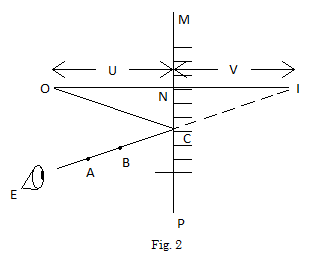
\includegraphics[width=6cm]{./img/2006-2-alt.png}
\end{center}

Fix a white sheet of paper on the soft board. Draw a line across the width at about the middle of the white sheep (MP). Draw line ONI perpendicular to MP.\\

Fix optical pin O to make ON = U = 3 cm. By using plasticine or otherwise, fix plane mirror along portion of MP with O in front of the mirror. With convenient position of eye, E, look into the mirror and fix optical pins A and B to be in line with image, I, of pin O.\\

Measure and record NI = V. Repeat procedure for U = 6 cm, 9 cm and 12 cm.

\begin{itemize}
\item[(a)] Tabulate your results as follows:\\[10pt]

\quad \quad \begin{tabular}{|l|c|c|c|c|} \hline
U (cm) &3&6&9&12 \\ \hline
V (cm) &&&& \\ \hline
\end{tabular} \\[10pt]

\item[(b)] Plot graph of U against V.
\item[(c)] Calculate slope, m, of the graph to the nearest whole number.
\item[(d)] State relationship between U and V.
\item[(e)] Write equation connecting U and V using numerical value of m with symbols U and V.
\item[(f)] From your equation give position of the image when object is touching the face of the mirror.
\end{itemize}

\end{enumerate}


\begin{enumerate}
\item[3.] You are required to determine the unknown resistance labeled X using a metre bridge circuit. Connect your circuit as shown below, where R is a resistance box, G is a galvanometer, J is a jockey and others are common circuit components.

\begin{center}
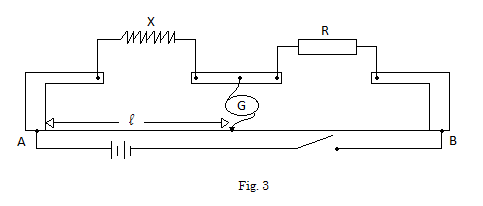
\includegraphics[width=14cm]{./img/2006-3-alt.png}
\end{center}

Procedure:\\

With R = 1 $\Omega$, obtain a balance point on a metre bridge wire AB using a jockey J. Note the length $l$ in centimetres. Repeat the experiment with R equal to 2 $\Omega$, 4 $\Omega$, 7 $\Omega$ and 10 $\Omega$.\\

Tabulate your results for R, $l$ and $^1/_l$.

\begin{itemize}
\item[(a)]
\begin{itemize}
\item[(i)] Plot a graph of R (vertical axis) against $^1/_l$ (horizontal axis).
\item[(ii)] Determine the slope S of your graph.
\item[(iii)] Using your graph, find the value of R for which $^1/_l = 0.02$.
\end{itemize}
\item[(b)] Read and record the intercept R$_0$ on the vertical axis.
\item[(c)] Given that,\\
\quad \quad R = $\cfrac{100\text{X}}{l}$ - X\\
Use the equation and your graph to determine the value of X.
\item[(d)] Comment on your results in (a)(iii), (b) and (c) above.
\end{itemize}

\end{enumerate}